\documentclass{TTP}

%--------------------------------------------- Basic packages (could be expanded by author)%
\usepackage{graphicx}
\usepackage[intlimits]{amsmath}
\usepackage{amssymb}
\usepackage{exscale}
\usepackage{hyperref}
\usepackage{times}
%\usepackage{xparse}
\usepackage{fontspec} 
\usepackage{subfigure}

\renewcommand{\large}{\fontsize{14}{18pt}\selectfont}
\renewcommand{\small}{\fontsize{11}{13.6pt}\selectfont}
\setmainfont{Times New Roman}
\setsansfont{Arial}

%--------------------------------------------- New commands for quick editing of the document%
\newcommand{\titleformat}{\sffamily\bfseries \large}            % <--- Doc. title
\newcommand{\authorformat}{\sffamily \large}              % <--- Authors
\newcommand{\keywordsformat}{\noindent \small \sffamily}        % <--- Kyewords
\newcommand{\abstractformat}{\noindent \textbf}           % <--- Abstract
\newcommand{\contentformat}{\rmfamily \normalsize\vspace{18pt}}     % <--- Main content
\newcommand{\email}{\sffamily \small \vspace{-8pt}}           % <--- E-mail
\renewcommand{\subsection}{\textbf} 

%--------------------------------------------- Make all internal and external links - black color%
\hypersetup{
    colorlinks,%
    citecolor=black,%
    filecolor=black,%
    linkcolor=black,%
    urlcolor=black
}

%--------------------------------------------- Set the basic parameters of the page. DO NOT CHANGE!%
\special{papersize=210mm,297mm}
\textheight=25.6cm

%--------------------------------------------- For the Publisher to Enter:

\begin{document}

\title{Icodrops Key Information Briefing ($v_time$)}

%\author{ FULL First Author \inst{1}$^{,\rm{a}}$ \textbf{,} FULL Second Author \inst{2}$^{,\rm{b}}$ and Last Author \inst{3}$^{,\rm{c}}$}
% \author{\authorformat FULL First Author \inst{1}$^{,\rm{a}}$\text{,} FULL Second Author \inst{,2}$^{,\rm{b}}$\text{,} and FULL Last Author \inst{3}$^{,\rm{c}}$}

% \institute{\sffamily Full address of first author, including country \and Full address of second author, including country\and
% List all distinct addresses in the same way}
\author{AgentSG}
\institute{ISS, NUS}

\maketitle

% \begin{center}
% \email{ $^{\rm a}$email, $^{\rm b}$email, $^{\rm c}$email}
% \end{center}


\section{Completion of financing targets}
According to the project data on Icodrops (nearly one year) we obtained, there are currently $v1_1$ projects. Among these $v1_1$ projects, $v1_2$ projects have completed their financing targets, accounting for $v1_3$, $v1_4$ projects did not complete their financing targets, accounting for $v1_5$, and the remaining $v1_6$ projects did not set financing targets, accounting for $v1_7$.
\begin{figure}[h]
  \centering
  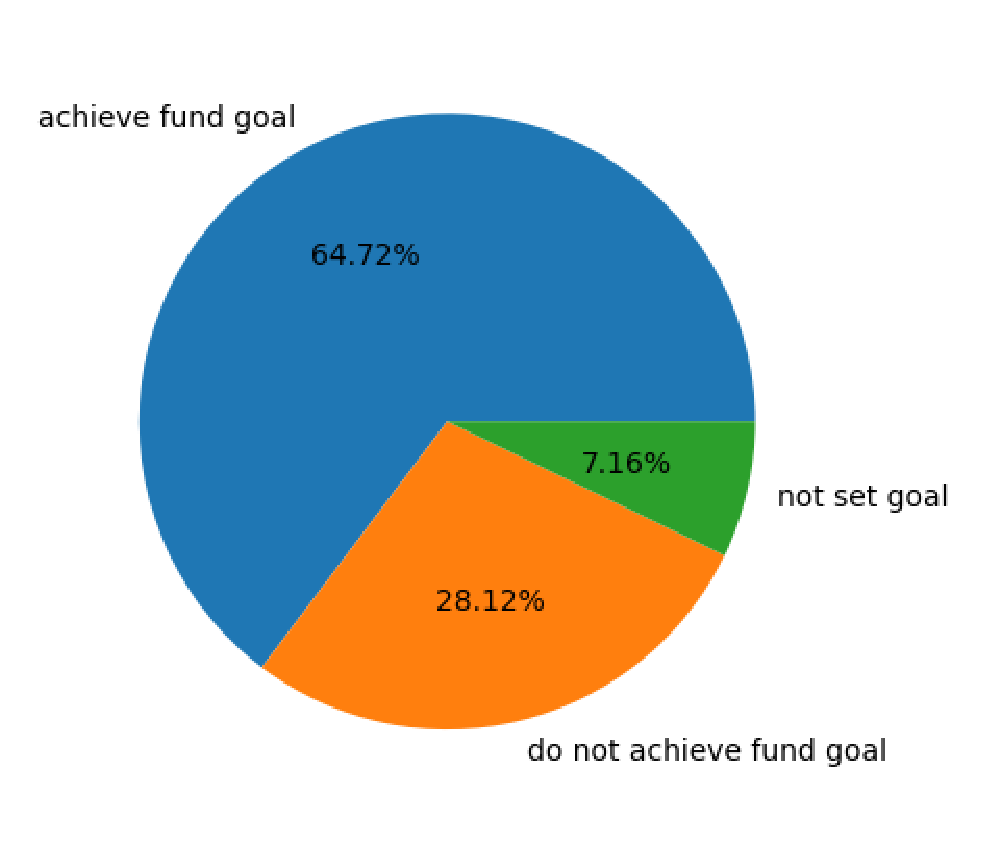
\includegraphics[width=8cm]{whether_achieve_fund_goal}
  \caption{whether achieve fund goal}
\end{figure}

\section{Total financing amount (monthly)}
From the data in the figure, we can see that in the last $v3_1$ months, $v3_2$ has the largest monthly financing amount and $v3_3$ has the least monthly financing amount. The difference between the two is $v3_4$. The three months with the highest financing amount are $v3_5$ ($v3_6$), $v3_7$ ($v3_8$), $v3_9$ ($v3_10$).
\begin{figure}[h]
  \centering
  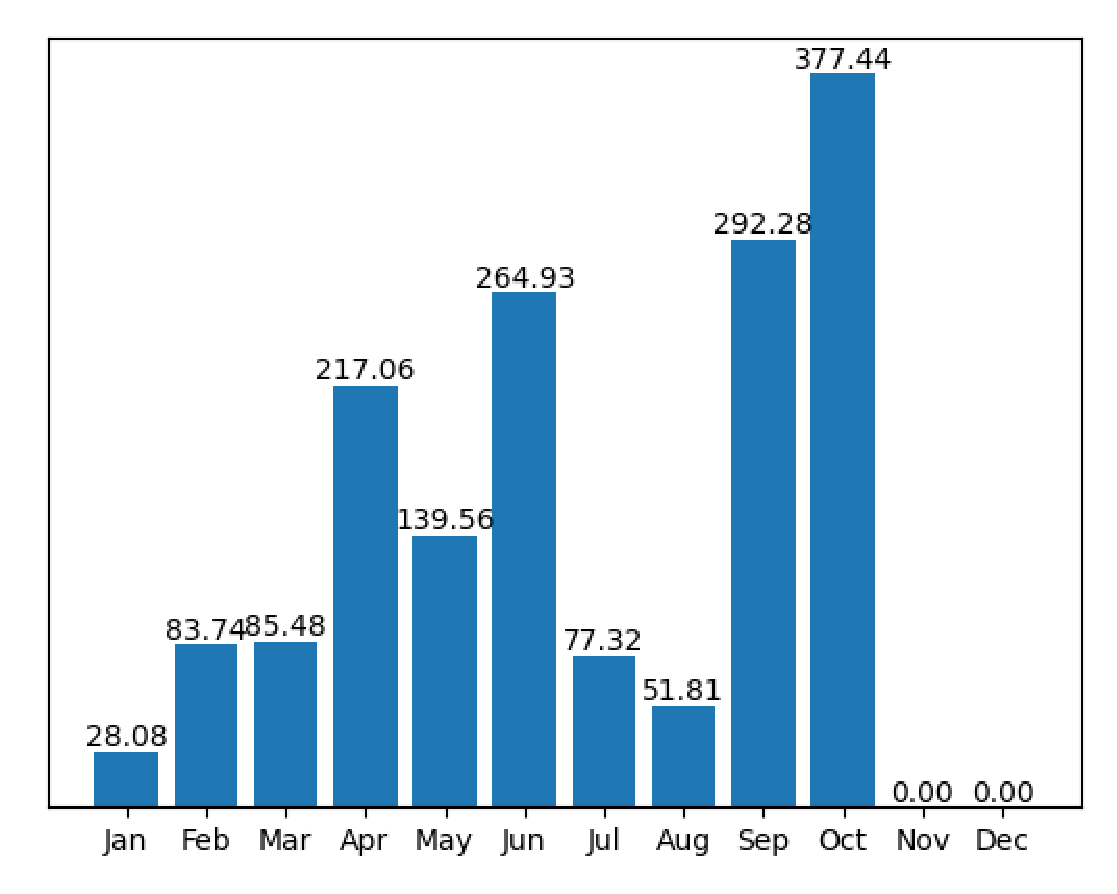
\includegraphics[width=8cm]{time_funding}
  \caption{funding amount according to time interval}
\end{figure}

\section{Distribution of financing amount}
From the recent (one year) project financing data we obtained on Icodrops, we can see that among all the projects involved in financing, there are $v2_1$ projects with a financing amount of less than 1 million US dollars, accounting for $v2_2$, the amount of project financing between US\$1 million and US\$3 million is $v2_3$, accounting for $v2_4$; $v2_5$ projects' financing amounts are between US\$3 million and US\$5 million, accounting for $v2_6$; $v2_7$ project financing The amount is between US\$5 million and US\$10 million, accounting for $v2_8$; $v2_9$ projects with financing amount exceeding US\$10 million, accounting for $v2_10$.
\begin{figure}[h]
  \centering
  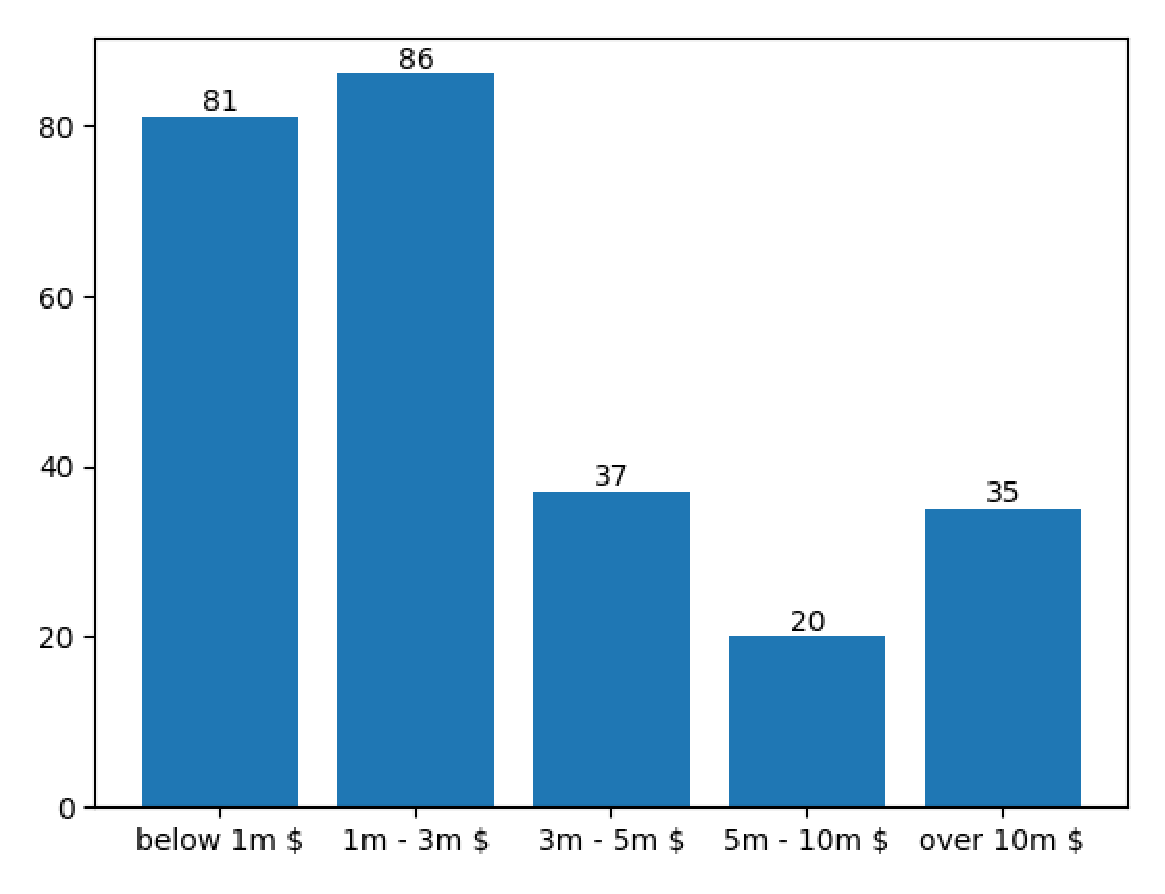
\includegraphics[width=8cm]{funding_range}
  \caption{funding range}
\end{figure}

\section{Token usage}
From the data in the figure below, we can see that in the past $v3_1$ months, most of the projects were used for ``$v4_1$'', the total financing amount was $v4_2$, accounting for $v4_3$, followed by that for ``$v4_4$'', the total financing is $v4_5$, the proportion is $v4_6$.
\begin{figure}[h]
  \centering
  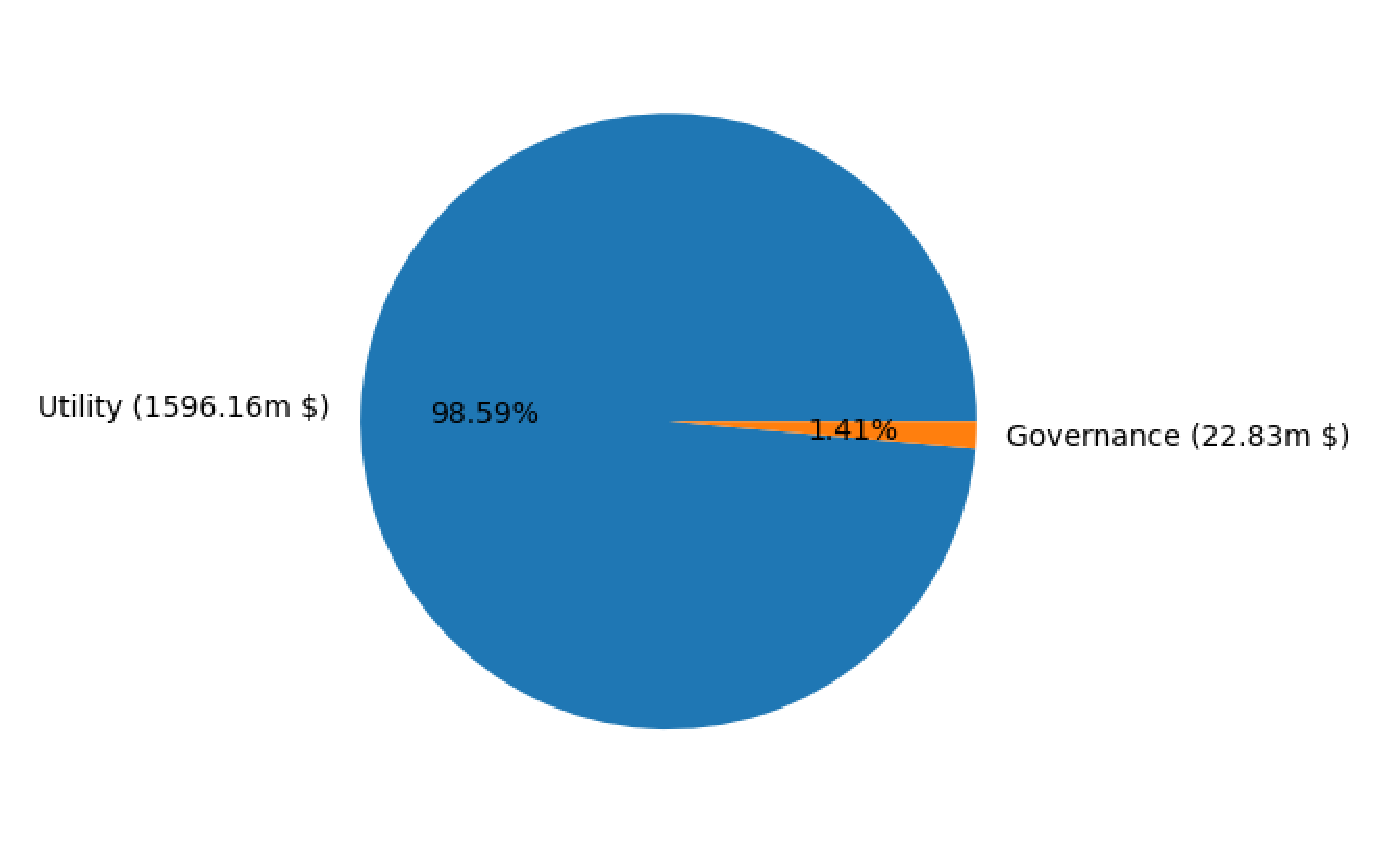
\includegraphics[width=10cm]{usage_funding}
  \caption{funding according to different usage}
\end{figure}

\newpage

\section{Need KYC or not}
Among all the above projects, $v5_1$ projects require kyc to be financed, accounting for $v5_2$; and $v5_3$ projects can participate in financing without kyc, accounting for $v5_4$.
\begin{figure}[h]
  \centering
  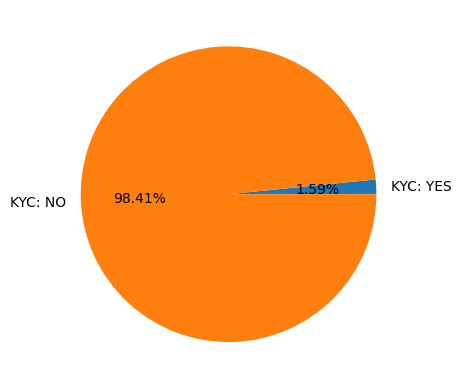
\includegraphics[width=8cm]{whether_kyc}
  \caption{KCY percentage}
\end{figure}

\end{document}